\documentclass[tikz,border=10pt]{standalone}
\usepackage{tikz}
\usetikzlibrary{shapes.geometric, arrows, positioning}
\begin{document}
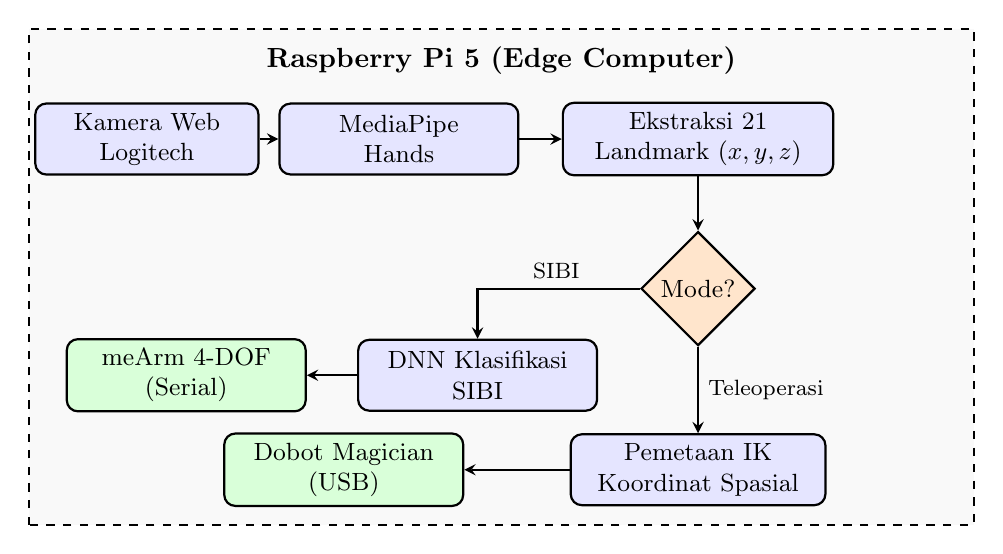
\begin{tikzpicture}[
    node distance=1.5cm,
    font=\small,
    box/.style={rectangle, draw=black, rounded corners, fill=blue!10, text centered, minimum height=0.9cm, text width=3.2cm, line width=0.8pt},
    decision/.style={diamond, draw=black, fill=orange!20, text centered, inner sep=2pt, line width=0.8pt},
    arrow/.style={thick, ->, >=stealth}
]
    % Container box for RPi 5
    \draw[dashed, fill=gray!5, line width=0.8pt] (-4.5, -4.5) rectangle (7.5, 1.8);
    \node at (1.5, 1.4) [font=\bfseries] {Raspberry Pi 5 (Edge Computer)};

    % Top nodes
    \node (cam) [box, text width=2.6cm] at (-3, 0.4) {Kamera Web\\Logitech};
    \node (mp) [box, text width=2.8cm] at (0.2, 0.4) {MediaPipe\\Hands};
    \node (ext) [box, text width=3.2cm] at (4.0, 0.4) {Ekstraksi 21\\Landmark $(x,y,z)$};

    % Decision node
    \node (dec) [decision] at (4.0, -1.5) {Mode?};

    % Branch 1: SIBI
    \node (dnn) [box, text width=2.8cm] at (1.2, -2.6) {DNN Klasifikasi\\SIBI};
    \node (mearm) [box, text width=2.8cm, fill=green!15] at (-2.5, -2.6) {meArm 4-DOF\\(Serial)};

    % Branch 2: Teleoperation
    \node (ik) [box, text width=3.0cm] at (4.0, -3.8) {Pemetaan IK\\Koordinat Spasial};
    \node (dobot) [box, text width=2.8cm, fill=green!15] at (-0.5, -3.8) {Dobot Magician\\(USB)};

    % Connections
    \draw [arrow] (cam) -- (mp);
    \draw [arrow] (mp) -- (ext);
    \draw [arrow] (ext) -- (dec);
    \draw [arrow] (dec) -| node[above, font=\footnotesize, xshift=1cm] {SIBI} (dnn);
    \draw [arrow] (dnn) -- (mearm);
    \draw [arrow] (dec) -- node[right, font=\footnotesize] {Teleoperasi} (ik);
    \draw [arrow] (ik) -- (dobot);
\end{tikzpicture}
\end{document}
